% Small moduli problems over Spec Z, after Grothendieck's working notes (folders 64, 83, 84, 85, 93). Standalone article for Hexagon.
% pdfLaTeX. Compile: latexmk -pdf article.tex (or tectonic -X compile article.tex).
\documentclass[11pt,a4paper]{amsart}
\usepackage[T1]{fontenc}
\usepackage[utf8]{inputenc}
\usepackage{lmodern,microtype,amssymb,mathtools,enumitem}
\usepackage[margin=2.7cm]{geometry}
\usepackage{tikz}
\usetikzlibrary{arrows.meta}
\usepackage[hidelinks]{hyperref}
\usepackage{xurl}
\emergencystretch=3em

\newtheorem{theorem}{Theorem}[section]
\newtheorem{proposition}[theorem]{Proposition}
\newtheorem{lemma}[theorem]{Lemma}
\newtheorem{corollary}[theorem]{Corollary}
\theoremstyle{definition}
\newtheorem{definition}[theorem]{Definition}
\newtheorem{statement}[theorem]{Statement}
\theoremstyle{remark}
\newtheorem{remark}[theorem]{Remark}
\newtheorem{example}[theorem]{Example}

\newcommand{\Z}{\mathbb Z}
\newcommand{\F}{\mathbb F}
\newcommand{\Q}{\mathbb Q}
\newcommand{\PP}{\mathbb P^1}
\newcommand{\PGL}{\mathrm{PGL}_2}
\newcommand{\GL}{\mathrm{GL}_2}
\newcommand{\Tr}{\operatorname{Tr}}
\newcommand{\id}{\mathrm{id}}
\newcommand{\fac}[1]{\href{https://grothendieck.umontpellier.fr/#1.pdf}{folder~#1}}
\newcommand{\lean}[1]{\texttt{\detokenize{#1}}}

\title[Small moduli over $\mathrm{Spec}\,\mathbb Z$]{Small moduli problems over $\operatorname{Spec}\mathbb Z$:\\ quadratic algebras, rotations in $\mathrm{PGL}_2$ and the integral Schwarzian,\\ after Grothendieck's working notes}
\author{Michel Hua}
\address{Commutator, Paris, France}
\email{michel@commutator.io}
\thanks{ORCID 0009-0002-8304-0683.}
\date{7 November 2026}
\subjclass[2020]{14D20; 11E16, 16H05, 20G15, 14H52, 53A55}
\keywords{quadratic algebras, product of quadratic algebras, Azumaya algebras, forms of PGL2, icosahedral group, Schwarzian derivative, Hasse derivatives, Lean}

\begin{document}
\begin{abstract}
Five folders of Grothendieck's notes from the 1980s, kept at the University of Montpellier, treat small moduli problems over $\operatorname{Spec}\Z$ without inverting $2$, $3$ or $5$. We prove the parts that can be done in coordinates over an arbitrary commutative ring, and correct the pages where they are wrong. Quadratic algebras are classified by triples $(L, \delta, T_0)$ when $2$ is a non-zero-divisor; their product has discriminant $\delta_1\delta_2$ and is the invariant algebra of $\sigma_1\otimes\sigma_2$ after every base change exactly when $2$, $b_1$, $b_2$ generate the unit ideal. The Hamilton--Cayley structures on $H\otimes H'$ form an affine line, and a structure is Azumaya exactly when $Q(t) = t^2 - bb't + b^2c' + b'^2c - 4cc'$ is a unit, in characteristic $2$ as well; $Q$ is the equation of the product of $H$ and $H'$. The invariant $A(g) = (\Tr g)^2/\det g - 2$ of $g \in \PGL$ detects the orders $3$ to $6$; we prove rigidity and a normal form for the group $G_2$, and show that in characteristic $5$ the octahedral configuration fills $\mathbb P^1(\F_5)$. The Schwarzian written with divided derivatives is a cocycle over $\Z$, and its vanishing forces a homography at Frobenius level $p$ for $p > 3$ and $p^2$ for $p = 2, 3$. The proofs are formalised in Lean.
\end{abstract}

\maketitle

\section{Introduction}

Five folders of Grothendieck's working notes, kept at the University of Montpellier, treat small moduli problems over an arbitrary base:
\begin{itemize}[leftmargin=1.5em]
\item \fac{84}, on binary quadratic forms and quadratic algebras, dated by the inventory from 1982 to about 1986;
\item \fac{83}, on Azumaya algebras of rank~$4$, with a part dated April 1986;
\item \fac{85}, \emph{2-polyèdres et 1-polygônes}, on regular polygons and polyhedra realised in forms of $\PGL$;
\item \fac{64}, \emph{Modules courbes elliptiques en caractéristiques $\neq 2$}, dated from 1980--1982;
\item \fac{93}, on the Schwarzian derivative and projective connections.
\end{itemize}
The method is the same throughout. Grothendieck writes the objects in coordinates over $\Z$, finds their invariants, and looks at what happens at the primes $2$, $3$ and~$5$ that the classical theory inverts. This paper states and proves the results of these folders that can be established in elementary terms. A statement is attributed to Grothendieck, with the page, when the page states it; otherwise it is said to be \emph{after} the page, and we say what was changed. The proofs are ours unless we say that we follow the page. Every proof given here is formalised in Lean~4 with Mathlib (Section~\ref{sec:lean}), except where we say otherwise. Grothendieck's global moduli statements need more than coordinates; we quote them as statements and say what we prove of them.

Throughout, $R$ is a commutative ring.

\section{Quadratic algebras and their product}\label{sec:quad}

Folder~84 works with the quadratic algebras $A(b,c) = R[U]/(U^2 + bU + c)$, without dividing by~$2$, and their discriminant $\delta(b,c) = b^2 - 4c$. With this sign, $\Tr(U) = -b$ and the canonical involution is $\sigma(U) = -b - U$.

Over a general affine base, page~45 describes a quadratic cover by an invertible module $L$ (for $A(b, c)$, $L$ is free, generated by the class of $U$ in $A/R$), an element $b \in L$ and an element $c \in L \otimes L$. The \emph{triple} of the cover is $(L, \delta, T_0)$, where $\delta = b \otimes b - 4c$ and $T_0$ is the class of $b$ in $L/2L$. A morphism of covers $(L, b, c) \to (L', b', c')$ is a pair $(\varphi, t)$, where $\varphi\colon L \to L'$ is an isomorphism, $t \in L'$, $\varphi(b) = b' + 2t$ and $(\varphi\otimes\varphi)(c) = c' + b'\otimes t + t\otimes t$. A morphism of triples is an isomorphism $\varphi$ with $(\varphi \otimes \varphi)(\delta) = \delta'$ and $\varphi(T_0) = T'_0$ in $L'/2L'$.

\begin{theorem}[Grothendieck, \fac{84}, pp.~45--53, affine base]\label{thm:triples}
Let $L$, $L'$ be invertible $R$-modules.
\begin{enumerate}
\item Over every $R$, the triple of a cover satisfies $T_0^2 \equiv \delta \bmod 4$, that is, $\tau\otimes\tau - \delta \in 4(L \otimes L)$ for a lift $\tau$ of $T_0$, and this does not depend on the lift. A morphism of covers is a morphism of triples, and every triple with $T_0^2 \equiv \delta \bmod 4$ is the triple of a cover with the same $L$.
\item If $2$ is a non-zero-divisor in $R$, every morphism of triples lifts to a unique morphism of covers. The functor from covers to triples is then an equivalence of groupoids. It commutes with base change $R \to S$ on objects and morphisms, over every $R$.
\item Over $\Z$, an integer $\delta$ is a discriminant iff $\delta \equiv 0, 1 \bmod 4$, and $A(b,c) \cong A(b',c')$ iff $\delta(b,c) = \delta(b',c')$ (p.~53).
\end{enumerate}
\end{theorem}

\begin{proof}[Sketch]
One has $b\otimes b - \delta = 4c$, and $(\tau - 2a)\otimes(\tau - 2a) - \tau\otimes\tau = 4(a\otimes a - \tau \otimes a)$, using that $L \otimes L$ is symmetric for $L$ invertible. If $\tau \otimes \tau - \delta = 4k$, the cover $(L, \tau, k)$ has triple $(L, \delta, T_0)$: this is the formula $c = (\tau^2 - \delta)/4$ of the page, written without division. When $2$ is regular, it is regular on the projective modules $L'$ and $L' \otimes L'$. The equation $\varphi(b) = b' + 2t$ then determines $t$, and the second condition on $(\varphi, t)$ follows from $(\varphi\otimes\varphi)(\delta) = \delta'$ after cancelling~$4$. Over $\Z$, $(b' - b)(b' + b) = 4(c' - c)$ forces $b' \equiv b \bmod 2$ once the discriminants agree.
\end{proof}

\begin{remark}
The hypothesis on $2$ in~(2) is needed. Over $\F_2$, $A(1,0) = \F_2 \times \F_2$ and $A(1,1) = \F_4$ have the same $b$ and the same $\delta = 1$, and they are not isomorphic, since a change of variable $V = U + t$ sends $(1, c)$ to $(1, c + t + t^2) = (1, c)$. Pages~49--52 reconstruct the algebra, its trace and its norm from the triple without division. In the free case, an element $y = a + eU$ has coordinates $\beta = \Tr y$ and $\gamma = e$, with $\beta \equiv \gamma b \bmod 2$, so that $y = (\beta + \gamma z)/2$ with $z = 2U + b$ and $z^2 = \delta$. The unit is $(2, 0)$, and
\[
2\beta(yy') = \beta\beta' + \gamma\gamma'\delta, \qquad 2\gamma(yy') = \beta\gamma' + \gamma\beta', \qquad 4N(y) = \beta^2 - \gamma^2\delta.
\]
For non-trivial $L$ we prove only that each of these divisions is legitimate; we do not prove that the pairs $(\beta, \gamma)$ form a ring isomorphic to the algebra of the cover.
\end{remark}

\subsection*{The product}
Page~63 defines the product of two quadratic algebras, ``sauf erreur'', by $b = b_1b_2$ and $4c = b^2 - \delta_1\delta_2$. The boxed formula writes $4c_1c_1$ where the computation gives $4c_1c_2$. Page~64 checks the generator.

\begin{proposition}[Grothendieck, \fac{84}, pp.~63, 64, 89, 102]\label{prop:product}
Let $u_i$ satisfy $u_i^2 + b_iu_i + c_i = 0$ in commutative $R$-algebras $A_i$, and put $b = b_1b_2$ and $c = c_1b_2^2 + c_2b_1^2 - 4c_1c_2$. In any commutative ring, with $Q_i = u_i^2 + b_iu_i + c_i$ and $u = 2u_1u_2 + b_1u_2 + b_2u_1$,
\[
u^2 + bu + c = b_2^2Q_1 + b_1^2Q_2 + 4(Q_1Q_2 - c_1Q_2 - c_2Q_1).
\]
Hence $\mathcal U = 2U_1U_2 + b_1U_2 + b_2U_1 \in A_1 \otimes_R A_2$ satisfies $\mathcal U^2 + b\,\mathcal U + c = 0$ and defines a morphism of $R$-algebras $A(b, c) \to A_1 \otimes A_2$. Moreover $b^2 - 4c = \delta_1\delta_2$.
\end{proposition}

\begin{proof}
Expand both sides; the identity is polynomial in $u_1, u_2, b_i, c_i$, with integer coefficients. The universal property of $A(b, c)$ gives the morphism.
\end{proof}

Voight studies this product over an arbitrary base scheme as the monoid of quadratic rings \cite{voight2016}. His Construction~3.12 is the same formula in the opposite sign convention; he credits the free affine case to Hahn and proves that the monoid structure is unique (Theorem~3.24). Part~(iii) of that theorem identifies the product with the invariants of $\sigma_1 \otimes \sigma_2$ when both algebras are separable. For quadratic algebras over rings in general, see Knus \cite{knus1991}. Pages~84--86 prove the identification with the invariants under a weaker hypothesis.

\begin{theorem}[Grothendieck, \fac{84}, pp.~84--86]\label{thm:coinv}
Let $A_i = A(b_i, c_i)$, with bases $(1, U_i)$, and let $E_i$ be the dual modules.
\begin{enumerate}
\item The map $E_1 \otimes E_2 \to E_1 * E_2$ of page~63 induces a well-defined map $(E_1 \otimes E_2)/\operatorname{Im}(\sigma_1\otimes\sigma_2 - \id) \to E_1 * E_2$, and this map is bijective iff $2R + b_1R + b_2R = R$.
\item If $2R + b_1R + b_2R = R$, the map $A(b, c) \to A_1 \otimes A_2$ of Proposition~\ref{prop:product} is injective with image $(A_1 \otimes A_2)^{\sigma_1\otimes\sigma_2}$. It has this property after every base change $R \to S$ iff $2R + b_1R + b_2R = R$.
\end{enumerate}
\end{theorem}

The page states the corollary~(2) with the hypothesis ``after every base change''. That hypothesis cannot be dropped: over $R = \Z[X]$ with $b_1 = X$ and $b_2 = 0$, the map is an isomorphism onto the invariants over $R$ itself, although $(2, X)$ is a proper ideal. The example is ours. In~(1), the kernel is generated by the Koszul relations of the unimodular row $(2, b_2, b_1)$. Geometrically, the condition says that at every point of residue characteristic~$2$ one of the two algebras is étale, since $A(b_i, c_i)$ is étale there iff $b_i$ is a unit.

Pages~65--79 build the product of extensions $0 \to L \to E \to M \to 0$ equipped with a $\chi$-splitting, for a fixed $\chi \in R$, by an amalgamated sum and without division. In the split case $E = M \oplus L$, a $\chi$-splitting is given by a linear map $b\colon M \to L$, through $\pi_b(\eta, \xi) = b(\eta) + \chi\xi$.

\begin{theorem}[Grothendieck, \fac{84}, pp.~65--79 and~123--131, split case over an affine base]\label{thm:chi}
Let $\chi \in R$, zero included.
\begin{enumerate}
\item Split extensions $M \oplus L$ with the $\chi$-splitting of $b\colon M \to L$, and morphisms $(f, \varphi, w)$ satisfying $\varphi b = b'f + \chi w$, form a symmetric monoidal category for the product $b_1 \otimes b_2$. A morphism is invertible as soon as $f$ and $\varphi$ are.
\item For $M = R$, the object $(R, L, b)$ is invertible for the product iff $L$ is an invertible module and $L = Rb + \chi L$ (margin of p.~79).
\item \emph{(After pp.~125, 127 and~169.)} If $\gamma\chi = 2$, the transvection $T_{\gamma b}$ identifies the ``pushed'' product, with $\chi$-splitting $\pi_b$, with the ``pulled'' product, with $\pi_{-b}$. For the unit objects, a map inducing the identity on $L$ and on $M$ and carrying one splitting to the other exists iff some $\gamma$ satisfies $\gamma\chi = 2$; over $\Z$ with $\chi = 4$ there is none.
\end{enumerate}
\end{theorem}

On an affine base every extension of $R$ by $L$ splits, and the amalgamated product of page~68 agrees with the product $b_1 \otimes b_2$; the non-split case over a scheme is not proved here.

\section{The line of twists and its degenerate locus}\label{sec:twist}

Folder~83 uses the opposite sign: $H = R[u]/(u^2 - bu + c)$ and $H' = R[v]/(v^2 - b'v + c')$, so that $\Tr u = b$ and $N(u) = c$. Pages~92--98 construct, for $(b, c, b', c', t) \in R^5$, the algebra $M = M(b, c; b', c'; t)$, free with basis $1, u, v, uv$, with $u^2 = bu - c$, $v^2 = b'v - c'$, $\Tr(uv) = t$ and the multiplication table of page~92. Pages~126--136 recover it as an algebra structure on $H \otimes H'$. Put
\[
Q(t) = t^2 - bb't + b^2c' + b'^2c - 4cc'.
\]

\begin{theorem}[after \fac{83}, pp.~81--84, 92--98 and~130--143]\label{thm:twist}
\leavevmode
\begin{enumerate}
\item For every $t$, $M$ is an associative unital $R$-algebra containing $H$ and $H'$. Every element satisfies $x^2 - \Tr(x)x + \det(x) = 0$, $\det$ is multiplicative, and $\Tr(uv) = t$. Conversely, let $A$ be an $R$-algebra whose elements satisfy $x^2 - T(x)x + N(x) = 0$ for a linear form $T$ and a function $N$, and let $u, v \in A$ have $T(u) = b$, $N(u) = c$, $T(v) = b'$, $N(v) = c'$. Then $x \mapsto x_0 + x_1u + x_2v + x_3uv$ is multiplicative from $M(b, c; b', c'; t)$ to $A$ for some $t$, unique if this map is injective. Distinct values of $t$ give distinct multiplications, so the structures form the affine line of $t$.
\item \emph{(Grothendieck, p.~98.)} $M$ is an Azumaya algebra iff $Q(t)$ is a unit. This holds over every commutative ring, characteristic $2$ included, and without hypothesis on $\delta = b^2 - 4c$ and $\delta' = b'^2 - 4c'$. Equivalently, the form $\det$ on $B = R1 + Ru + Rv$ has invertible half-discriminant, which equals $-Q(t)$.
\item The discriminant of the trace form of $M$ in the basis $(1, u, v, uv)$ is $-Q(t)^2$. The polynomial $Q$ has discriminant $\delta\delta'$ and is invariant under $t \mapsto bb' - t$, and the degenerate locus $\widetilde S = \operatorname{Spec} R[t]/(Q)$ is free of rank $2$ over $R$.
\item In $H \otimes H'$, the element $u * v = b'u + bv - 2u \otimes v$ satisfies $Q(u * v) = 0$, which gives a morphism $R[t]/(Q) \to H \otimes H'$. The canonical involution of either factor sends $u * v$ to $bb' - u * v$. For characters $\varphi$, $\varphi'$ of $H$, $H'$ with values in a commutative $R$-algebra $K$, the element $b'\varphi(u) + b\varphi'(v) - 2\varphi(u)\varphi'(v)$ is a root of $Q$ in $K$.
\end{enumerate}
\end{theorem}

\begin{proof}[Sketch]
(1) Each axiom is a polynomial identity in the coordinates; for the converse, Hamilton--Cayley applied to $u + v$ gives $vu = (t - bb') + b'u + bv - uv$ with $t = bb' + c + c' - N(u + v)$, and the rest of the table follows by associativity. (2) $M$ is free, so it is Azumaya iff the sandwich map $M \otimes M^{\mathrm{op}} \to \operatorname{End}_R M$ is bijective, that is, iff its $16 \times 16$ determinant $D$ is a unit. Composing with the trace pairing of $\operatorname{End}_R M$ gives the Kronecker square of the trace form of $M$, so $\pm D^2 = (-Q^2)^8 = Q^{16}$. The argument uses only the determinant of the trace form, not its non-degeneracy, so it holds in characteristic~$2$. (4) In $H \otimes H'$, with $U = u \otimes 1$ and $V = 1 \otimes v$,
\[
Q(b'U + bV - 2UV) = (2V - b')^2(U^2 - bU + c) + (b^2 - 4c)(V^2 - b'V + c'),
\]
and the right-hand side vanishes.
\end{proof}

Two misprints on the pages are corrected here. Page~138 writes the constant term of $Q$ as $b^2b' + b'^2b - 4cc'$, and page~143 writes $\det(u * v) = b^2c + b'^2c' - 4cc'$; both should read $b^2c' + b'^2c - 4cc'$. For $b = c = b' = c' = 0$, $M(0,0;0,0;t)$ is Azumaya iff $t$ is a unit, as page~97 says.

\begin{figure}[ht]
\centering
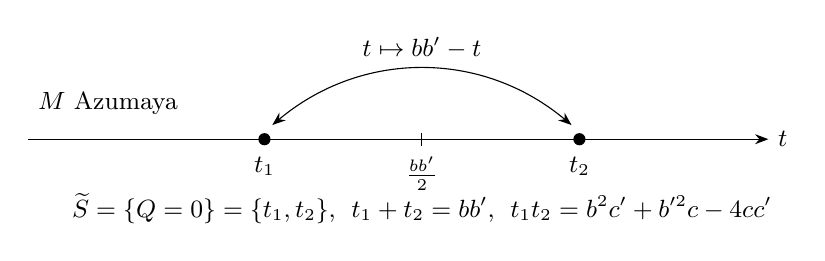
\begin{tikzpicture}[x=1cm, y=1cm, every node/.style={font=\small}]
\draw[-{Stealth}] (-4.6,0) -- (4.8,0) node[right] {$t$};
\fill (-1.6,0) circle (2.2pt); \fill (2.4,0) circle (2.2pt);
\node[below=3pt] at (-1.6,0) {$t_1$}; \node[below=3pt] at (2.4,0) {$t_2$};
\draw (0.4,0.08) -- (0.4,-0.08); \node[below=3pt] at (0.4,0) {$\tfrac{bb'}{2}$};
\draw[{Stealth}-{Stealth}] (-1.5,0.18) to[bend left=40] node[above] {$t \mapsto bb' - t$} (2.3,0.18);
\node[below=16pt] at (0.4,0) {$\widetilde S = \{Q = 0\} = \{t_1, t_2\}$, $\;t_1 + t_2 = bb'$, $\;t_1t_2 = b^2c' + b'^2c - 4cc'$};
\node[anchor=west] at (-4.6,0.45) {$M$ Azumaya};
\end{tikzpicture}
\caption{The line of twists over a field, when $Q$ has two roots. Away from $t_1$ and $t_2$ the algebra $M(b, c; b', c'; t)$ is Azumaya. The canonical involutions exchange the two degenerate points, and the two roots coincide iff $\delta\delta' = 0$.}
\label{fig:twist}
\end{figure}

Point~(4) links this section with Section~\ref{sec:quad}. In the notation of folder~84, $H = A(-b, c)$ and $H' = A(-b', c')$. The generator of Proposition~\ref{prop:product} is then $\mathcal U = 2UV - bV - b'U = -(u * v)$, and the product is $A(bb', b^2c' + b'^2c - 4cc')$, with equation $P(T) = T^2 + bb'T + b^2c' + b'^2c - 4cc'$. Since $Q(t) = P(-t)$, the map $t \mapsto -\mathcal U$ identifies $R[t]/(Q)$ with the product of $H$ and $H'$, and the morphism of~(4) with the canonical morphism of Proposition~\ref{prop:product}. In Voight's convention, $Q$ is exactly the polynomial of his Construction~3.12. So the non-Azumaya locus of the line of twists is the spectrum of the product $H * H'$, as pages~137--143 assert. Pages~137--143 also identify $\widetilde S$ with the quotient of $X \times_S X'$ by $\sigma \times \sigma'$. We prove only the algebraic core of that statement: by Theorem~\ref{thm:coinv}, the invariants of $\sigma\otimes\sigma'$ in $H \otimes H'$ are $R[u * v]$ when $2$, $b$, $b'$ generate the unit ideal.

\section{Rotations in forms of \texorpdfstring{$\mathrm{PGL}_2$}{PGL2}}\label{sec:pgl}

Folder~85 realises polygons and polyhedra in a form of $\PGL$ over a base by means of a single invariant. For $g \in M_2(R)$ with $\det g$ invertible, put
\[
A(g) = \frac{(\Tr g)^2}{\det g} - 2.
\]
It depends only on the image of $g$ in $\PGL(R)$, and it equals $\zeta + \zeta^{-1}$ when the eigenvalues of $g$ have ratio $\zeta$. Call $g$ \emph{nowhere scalar} if its image in $M_2(R/\mathfrak m)$ is not scalar for every maximal ideal $\mathfrak m$; equivalently, the off-diagonal entries and the difference of the diagonal entries generate the unit ideal. For $\nu \ge 2$, say that $g$ has \emph{order $\nu$ at every point} if $g^\nu$ is scalar and $g^m$ is nowhere scalar for every divisor $m$ of $\nu$ with $1 \le m < \nu$. For $\nu$ prime and $g$ nowhere scalar, this just says that $g^\nu$ is scalar.

\begin{theorem}[after \fac{85}, pp.~6--7, 29--31 and~40]\label{thm:orders}
Let $g \in M_2(R)$ be nowhere scalar, with trace $t$, invertible determinant $d$, and $\alpha = A(g)$.
\begin{enumerate}
\item With $x_0 = 0$, $x_1 = 1$, $x_{n+2} = tx_{n+1} - dx_n$, one has $g^{n+1} = x_{n+1}g - dx_n$, and $g^{n+1}$ is scalar iff $x_{n+1} = 0$. In particular $g^2$ is scalar iff $t = 0$, that is, $\alpha = -2$.
\item $g^3$ is scalar iff $\alpha = -1$. The element $g$ has order $4$ at every point iff $\alpha = 0$ and $2$ is invertible, and order $6$ at every point iff $\alpha = 1$ and $6$ is invertible.
\item $g^5$ is scalar iff $\alpha^2 + \alpha - 1 = 0$. Moreover $A(g^2) = A(g)^2 - 2$, so that $A(g^2) = -1 - A(g)$ in that case (the corollary of page~40).
\end{enumerate}
The implication ``$\alpha^2 + \alpha - 1 = 0 \Rightarrow g^5$ scalar'' holds for every $g$ with invertible determinant.
\end{theorem}

\begin{proof}
(1) is Cayley--Hamilton, $g^2 = tg - d$, together with the fact that $xg + y$ is scalar iff $x = 0$ when $g$ is nowhere scalar. Since $t^2 = (\alpha + 2)d$, induction gives $x_{2k+1} = d^kP_{2k+1}(\alpha)$ and $x_{2k+2} = t\,d^kP_{2k+2}(\alpha)$, where $P_0 = 0$, $P_1 = 1$, $P_{n+2} = P_{n+1} - P_n$ for $n$ even and $P_{n+2} = (\alpha + 2)P_{n+1} - P_n$ for $n$ odd. Thus $P_3 = \alpha + 1$, $P_4 = \alpha$, $P_5 = \alpha^2 + \alpha - 1$ and $P_6 = \alpha^2 - 1$, which gives (2) and (3). For order $4$, $g^2$ is nowhere scalar iff $x_2 = t$ is invertible, and then $\alpha = 0$ gives $t^2 = 2d$, so $2$ is invertible. For order $6$, $t$ and $x_3 = d(\alpha + 1)$ must be invertible, so $\alpha = 1$, and then $t^2 = 3d$ and $\alpha + 1 = 2$ make $6$ invertible. Finally $A(g^2) = (t^2 - 2d)^2/d^2 - 2 = A(g)^2 - 2$.
\end{proof}

\begin{figure}[ht]
\centering
\begin{tikzpicture}[x=1.75cm, y=1.75cm, every node/.style={font=\small}]
\draw[-{Stealth}] (-2.45,0) -- (2.6,0) node[right] {$A$};
\draw[densely dotted] (2,0) arc (0:180:2);
\foreach \ang/\lab in {120/3, 90/4, 72/5, 144/5, 60/6} {
  \draw[densely dashed, gray] ({2*cos(\ang)},0) -- ({2*cos(\ang)},{2*sin(\ang)});
  \fill ({2*cos(\ang)},{2*sin(\ang)}) circle (1.8pt);
  \node at ({2.22*cos(\ang)},{2.22*sin(\ang)+0.02}) {$\lab$};
  \fill ({2*cos(\ang)},0) circle (1.4pt);
}
\fill (2,0) circle (1.8pt); \fill (-2,0) circle (1.8pt);
\node[above right=1pt] at (2,0) {$1$}; \node[above left=1pt] at (-2,0) {$2$};
\node[below=2pt] at (-2,0) {$-2$}; \node[below=2pt] at (-1,0) {$-1$};
\node[below=2pt] at (0,0) {$0$}; \node[below=2pt] at (1,0) {$1$}; \node[below=2pt] at (2,0) {$2$};
\node[below=13pt] at ({2*cos(144)},0) {$\tfrac{-1-\sqrt5}{2}$};
\node[below=13pt] at ({2*cos(72)},0) {$\tfrac{-1+\sqrt5}{2}$};
\end{tikzpicture}
\caption{Reading the order on $A(g)$. Over $\mathbb C$, a rotation by the angle $\theta$ has $A = 2\cos\theta$. The points of the upper half circle are labelled by the order of the rotation, and their projections are the values of $A$: $-2$ for involutions, $-1$, $0$ and $1$ for orders $3$, $4$ and $6$, and the two roots of $A^2 + A - 1$ for order $5$. Theorem~\ref{thm:orders} proves the same reading over any ring, with the conditions on $2$ and $6$ for orders $4$ and~$6$.}
\label{fig:orders}
\end{figure}

\begin{example}[\fac{85}, p.~40]
Over $\Z[\zeta_5]$, the matrices $s = \bigl(\begin{smallmatrix} 0 & -1 \\ 1 & 0\end{smallmatrix}\bigr)$ and $p = \bigl(\begin{smallmatrix} \zeta & 1 \\ 0 & \zeta^4\end{smallmatrix}\bigr)$ satisfy $s^2 = -1$, $(sp)^3 = -1$ and $p^5$ scalar, and $A(p) = \zeta^2 + \zeta^3$ is a root of $T^2 + T - 1$. The matrices $s$, $p$ and $sp$ are nowhere scalar. Since $\langle s, p \mid s^2, (sp)^3, p^5\rangle$ is a presentation of $\mathfrak A_5$, they define a homomorphism $\mathfrak A_5 \to \PGL(\Z[\zeta_5])$. It is injective on every fibre, because its image there is a non-trivial quotient of the simple group $\mathfrak A_5$. This last step is not formalised. In characteristic~$5$, $\zeta = 1$ and $p$ is unipotent, with $A(p) = 2$, a double root of $T^2 + T - 1 = (T - 2)^2$.
\end{example}

Page~40 states the following.

\begin{statement}[Grothendieck, \fac{85}, p.~40]\label{st:a5}
For a form $G$ of $\PGL$ over a scheme $S$ and a monomorphism $\varphi\colon\mathfrak A_5 \to G$, the element $\alpha(\varphi) = A(\varphi(\pi))$, $\pi$ a $5$-cycle, satisfies $\alpha^2 + \alpha - 1 = 0$. The category of pairs $(G, \varphi)$ is rigid, and its functor of isomorphism classes is represented by $\operatorname{Spec}\Z[T]/(T^2 + T - 1)$.
\end{statement}

Theorem~\ref{thm:orders}(3) proves the first assertion over every base, for matrices. We do not prove rigidity or representability. Together they would say that, over any base, including residue characteristics $2$, $3$ and~$5$, a pair $(G, \varphi)$ is determined up to unique isomorphism by the root $\alpha$. Forms of $\PGL$ cannot be avoided here. By Beauville's Proposition~1.1 \cite{beauville2010}, for a field $K$ of characteristic prime to $60$, $\PGL(K)$ contains $\mathfrak A_5$ iff $-1$ is a sum of two squares in $K$ and $5$ is a square. So the split group over $\mathbb R$, or over $\Q(\sqrt 5)$, contains no $\mathfrak A_5$.

\subsection*{The group $G_2$}
Pages~4--7 treat homomorphisms into $\PGL(R)$ of the group $G_2 = \langle\tau_0, \tau_1, \tau_2 \mid \tau_i^2, (\tau_0\tau_2)^2\rangle$. The notation is the page's; $G_2$ is the Coxeter group with string diagram and unspecified orders of $\tau_0\tau_1$ and $\tau_1\tau_2$, not the exceptional group. Such a homomorphism is given by matrices $\tau_i$ with invertible determinants and with $\tau_i^2$ and $(\tau_0\tau_2)^2$ scalar. Put $\rho_0 = \tau_0\tau_1$, $\rho_1 = \tau_1\tau_2$, $\alpha_i = A(\rho_i)$, and $\Delta = (\alpha_0 + 2)(\alpha_1 + 2)(\alpha_0 + \alpha_1)$. Over a field, condition $(*)$ of page~4 says that $\rho_0^2$ and $\rho_1^2$ are not scalar and that $\rho_0\rho_1$ is not a scalar multiple of $\rho_1\rho_0$. We say that $(*)$ holds at every point if it holds for the images of the $\tau_i$ in $M_2(R/\mathfrak m)$ for every maximal ideal $\mathfrak m$.

\begin{theorem}[after \fac{85}, pp.~4--7]\label{thm:g2}
\leavevmode
\begin{enumerate}
\item $(*)$ holds at every point iff $\tau_0$, $\tau_1$, $\tau_2$ and $\tau_0\tau_2$ are traceless and $\Delta$ is invertible. Each factor of $\Delta$ corresponds to one condition of $(*)$.
\item \emph{Rigidity.} Under these conditions, if $g \in \GL(R)$ and $\mu_i \in R$ satisfy $g\tau_i = \mu_i\tau_ig$ for $i = 0, 1, 2$, then $g$ is scalar.
\item \emph{Normal form.} For every $(\alpha_0, \alpha_1)$ with $\Delta$ invertible, explicit traceless matrices with these invariants and with $(*)$ at every point exist over $R[T]/(T^2 - \alpha_0T + 1)$, which is free of rank~$2$ over $R$. Over a field containing a root of $T^2 - \alpha_0T + 1$, two triples with the same invariants are conjugate in $\PGL$.
\end{enumerate}
\end{theorem}

\begin{proof}[Sketch]
For traceless $\tau_i$ with $\Tr(\tau_0\tau_2) = 0$, write $t_{01} = \Tr\rho_0$, $t_{12} = \Tr\rho_1$, $T = \Tr(\tau_0\tau_1\tau_2)$ and $d_i = \det\tau_i$. Then $\alpha_0 + 2 = t_{01}^2/(d_0d_1)$, $\alpha_1 + 2 = t_{12}^2/(d_1d_2)$, $\rho_0\rho_1 - \rho_1\rho_0 = -T\tau_1$ and $\alpha_0 + \alpha_1 = -T^2/(d_0d_1d_2)$, so $\Delta$ is invertible iff $t_{01}$, $t_{12}$ and $T$ are. Conversely, an involution $\tau$ that is nowhere scalar has $\tau^2 = (\Tr\tau)\tau - \det\tau$ scalar, which forces $\Tr\tau = 0$. For~(2), the traces give $\mu_0\mu_1 = \mu_1\mu_2 = 1$, so $g$ commutes with $\rho_0$ and $\rho_1$; then $g = p + q\rho_0$, and $qT\tau_1 = 0$ forces $q = 0$.
\end{proof}

The moduli statement that follows is the edition's reformulation of pages~4--7 and is not proved here: homomorphisms of $G_2$ into forms of $\PGL$ satisfying $(*)$ in every fibre would be classified by the complement of the three lines $\Delta = 0$ in $\mathbb A^2_\Z$.

\subsection*{Octahedral configurations}
Folder~64 considers a faithful action of the Klein group on $\PP$, locally $z \mapsto -z$, $z \mapsto 1/z$, whose axes form the octahedral configuration $\Delta = \{0, \infty, \pm1, \pm i\}$. To identify $\operatorname{Aut}(\PP, \Delta)$ with the rotation group of the octahedron, page~48 computes the fixer of the two non-opposite vertices $\infty$ and $-1$. Its elements are the maps $z \mapsto az + (a - 1)$.

\begin{theorem}[Grothendieck, \fac{64}, p.~48]\label{thm:fixer}
Let $K$ be a field with $2 \ne 0$ and $i^2 = -1$. If $z \mapsto az + (a - 1)$ maps $\{0, 1, i, -i\}$ into itself, then $5(a - 1) = 0$. In particular, if $5 \ne 0$ in $K$, the fixer of $\infty$ and $-1$ in $\operatorname{Aut}(\PP_K, \Delta)$ is trivial.
\end{theorem}

\begin{proof}
The four points are distinct because $2 \ne 0$. If $a = 0$, the map sends $0$ to $-1$, which is not one of them. Otherwise the map is injective, so it permutes the four points and preserves their sum, which is $1$. The sum of the images is $a + 4(a - 1) = 5a - 4$, so $5a - 4 = 1$.
\end{proof}

The margin restricts the computation to ``car.~$\ne 3$ et $5$''. The proof shows that characteristic~$3$ needs no special case. In characteristic~$5$ the identification fails. There $i = \pm 2$, and $z \mapsto 2z + 1$ permutes $\{0, 1, i, -i\}$. Over $\F_5$ the configuration $\Delta$ is all of $\PP(\F_5)$, so every one of the $120$ elements of $\PGL(\F_5)$ preserves it, and the fixer of $\infty$ and $-1$ consists of the identity and the maps $z \mapsto az + (a - 1)$ for $a = 2, 3, 4$ (Figure~\ref{fig:octa}).

\begin{figure}[ht]
\centering
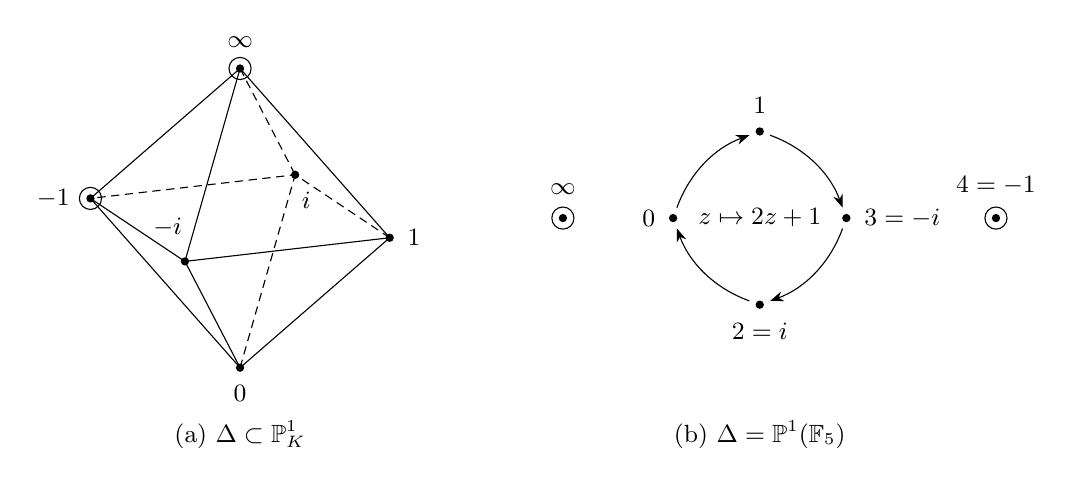
\begin{tikzpicture}[x=1cm, y=1cm, every node/.style={font=\small}]
\begin{scope}
\coordinate (inf) at (0,1.9); \coordinate (z) at (0,-1.9);
\coordinate (p1) at (1.9,-0.25); \coordinate (m1) at (-1.9,0.25);
\coordinate (pi) at (0.7,0.55); \coordinate (mi) at (-0.7,-0.55);
\draw (m1)--(mi)--(p1); \draw[densely dashed] (p1)--(pi)--(m1);
\foreach \v in {m1,mi,p1} { \draw (inf)--(\v); \draw (z)--(\v); }
\draw[densely dashed] (inf)--(pi); \draw[densely dashed] (z)--(pi);
\foreach \v in {inf,z,p1,m1,pi,mi} \fill (\v) circle (1.5pt);
\draw (inf) circle (4pt); \draw (m1) circle (4pt);
\node[above=4pt] at (inf) {$\infty$}; \node[below=3pt] at (z) {$0$};
\node[right=3pt] at (p1) {$1$}; \node[left=4pt] at (m1) {$-1$};
\node at (0.84,0.22) {$i$}; \node at (-0.92,-0.12) {$-i$};
\node at (0,-2.75) {(a) $\Delta \subset \PP_K$};
\end{scope}
\begin{scope}[xshift=6.6cm]
\coordinate (a0) at (-1.1,0); \coordinate (a1) at (0,1.1);
\coordinate (a3) at (1.1,0); \coordinate (a2) at (0,-1.1);
\coordinate (ainf) at (-2.5,0); \coordinate (a4) at (3.0,0);
\foreach \v in {a0,a1,a2,a3,ainf,a4} \fill (\v) circle (1.5pt);
\draw (ainf) circle (4pt); \draw (a4) circle (4pt);
\draw[-{Stealth}, shorten <=4pt, shorten >=4pt] (a0) to[bend left=25] (a1);
\draw[-{Stealth}, shorten <=4pt, shorten >=4pt] (a1) to[bend left=25] (a3);
\draw[-{Stealth}, shorten <=4pt, shorten >=4pt] (a3) to[bend left=25] (a2);
\draw[-{Stealth}, shorten <=4pt, shorten >=4pt] (a2) to[bend left=25] (a0);
\node[left=3pt] at (a0) {$0$}; \node[above=3pt] at (a1) {$1$};
\node[right=3pt] at (a3) {$3 = -i$}; \node[below=3pt] at (a2) {$2 = i$};
\node[above=5pt] at (ainf) {$\infty$}; \node[above=5pt] at (a4) {$4 = -1$};
\node at (0,0) {$z \mapsto 2z + 1$};
\node at (0,-2.75) {(b) $\Delta = \PP(\F_5)$};
\end{scope}
\end{tikzpicture}
\caption{(a) The octahedral configuration; opposite vertices are $0$ and $\infty$, $1$ and $-1$, $i$ and $-i$. The fixer of the circled vertices $\infty$ and $-1$ permutes the other four, and Theorem~\ref{thm:fixer} shows it is trivial when $5 \ne 0$. (b) Over $\F_5$, with $i = 2$, the six vertices are the six points of $\PP(\F_5)$, and $z \mapsto 2z + 1$ fixes $\infty$ and $-1$ and cycles the other four.}
\label{fig:octa}
\end{figure}

Pages~44--52 state that, over a base whose residue characteristics are $\ne 2$, three sets correspond bijectively: the subgroup schemes of $\operatorname{Aut}_S(X)$ locally isomorphic to $(\Z/2)^2$, those locally isomorphic to $\mathfrak S_4$, and the regular octahedral configurations. Where the pages identify $\operatorname{Aut}_S(X, \Delta)$ with the octahedral rotation group, the example above shows that $5$ must be invertible. Over a field, Beauville's Proposition~1.1 \cite{beauville2010} says that $\PGL(K)$ contains $\mathfrak S_4$ iff $-1$ is a sum of two squares, for $K$ of characteristic prime to~$6$; in characteristic $5$ this subgroup exists, but it is not the full stabiliser of $\Delta$. Pages~74--91 describe the moduli of elliptic curves with a level-$2$ structure and a ``Legendre pinning'' over $\Z[1/2]$ by $U_{0,3} \times \mu_4^*$. Antieau and Meier prove a related statement without the pinning: the parameter space of Legendre curves $\mathbb A^1_{\Z[1/2]} - \{0, 1\}$ is a $C_2$-torsor over the stack $\mathcal M(2)$ of elliptic curves with full level-$2$ structure \cite[Definition~4.4 and Proposition~4.5, arXiv numbering]{antieaumeier2020}. Neither of the folder's relative statements is proved here.

\section{The Schwarzian with divided derivatives}\label{sec:schwarz}

Folder~93 studies the Schwarzian derivative and projective connections on a smooth curve over a base. For two uniformisers $t$, $s$, the classical Schwarzian difference is $G(t, s) = \bigl(-2s'''/s' + 3(s''/s')^2\bigr)\,dt^2$. Page~72 replaces the derivatives by the divided operators $D^{(i)} = \frac{1}{i!}\frac{d^i}{dt^i}$ of Hasse and Schmidt \cite{hasseschmidt1937}, observes that the coefficients $2$ and $3$ of $G$ prevent this, and takes $G_0 = G/12$:
\[
G_0(t, s) = -\frac{D^{(3)}s}{D^{(1)}s} + \Bigl(\frac{D^{(2)}s}{D^{(1)}s}\Bigr)^2.
\]
Put $N(s) = (D^{(2)}s)^2 - D^{(1)}s\cdot D^{(3)}s$, so that $G_0(s) = N(s)/(D^{(1)}s)^2$. We work in the local model $R[X]$, with $X$ in the role of $t$, and in its quotients.

\begin{theorem}[Grothendieck, \fac{93}, pp.~71--73 and~115--123]\label{thm:schwarz}
\leavevmode
\begin{enumerate}
\item $G = 12\,G_0$, and $G_0$ is defined over every base, characteristics $2$ and $3$ included.
\item \emph{Cocycle.} For polynomials $s$, $u$, one has $N(s \circ u) = (N(s)\circ u)(D^{(1)}u)^4 + \bigl((D^{(1)}s)\circ u\bigr)^2N(u)$. If $D^{(1)}s$ and $D^{(1)}u$ are invertible, $G_0(s \circ u) = (G_0(s)\circ u)(D^{(1)}u)^2 + G_0(u)$.
\item \emph{Homographies.} If $a, b, c, d \in R$, $cX + d$ is invertible and $s(cX + d) = aX + b$, then $G_0(s) = 0$.
\item \emph{Killed functions} (margin of p.~121). In characteristic $p$, a polynomial is killed by $D^{(1)}$, $D^{(2)}$ and $D^{(3)}$ iff it is a polynomial in $X^p$ for $p > 3$, in $X^4$ for $p = 2$, and in $X^9$ for $p = 3$.
\item \emph{Rigidity.} Let $A$ be a local ring of characteristic $p$, let $e = 1$ if $p > 3$ and $e = 2$ if $p = 2, 3$, and let $\alpha \in A$. If $s \in A[T]/(T^{p^e} - \alpha)$ has $D^{(1)}s$ invertible and $G_0(t, s) = 0$, then $s = (at + b)/(ct + d)$ with $a, b, c, d \in A$ and $ct + d$ invertible. The same holds for any $A$ of characteristic $p$ with $\operatorname{Pic}(A) = 0$.
\end{enumerate}
\end{theorem}

\begin{proof}[Sketch]
(1)--(3) are identities of the divided-power calculus. For (3), Leibniz applied to $sq = p$, with $q = cX + d$ and $p = aX + b$, gives $q^2N(s) = 0$. For (5) with $\alpha = 0$, take $d = 1$, $c = -s_2/s_1$, $b = s_0$, $a = s_1 + cs_0$ and $r = s\,(cX + 1)$. If $X^{j+3}$ divides $r - (aX + b)$, the coefficient of $X^j$ in $(cX + 1)N(s)$ is $-\binom{j+3}{3}s_1r_{j+3}$. Induction on $j$ then gives $X^n \mid s(cX + 1) - (aX + b)$ as long as $\binom k3$ is invertible for $3 \le k < n$. This holds for $n = p$ ($p > 3$), $n = 4$ ($p = 2$, where only $\binom33 = 1$ occurs) and $n = 9$ ($p = 3$, where $\binom k3 = 1, 4, 10, 20, 35, 56$ for $k = 3, \dots, 8$). For general $\alpha$, let $q = p^e$ and $B = A[T]/(T^q - \alpha)$, where $T^q - \alpha = (T - \beta)^q$ with $\beta$ the class of~$T$. The Taylor map $\theta(f) = f(\beta + Y)$ reduces the question to the case $\alpha = 0$ over $B$. This gives the osculating homography at $\beta$, with coefficients in~$B$. Its coefficient vector $v$ satisfies $(cY + 1)\,\theta(v) \equiv v \bmod Y^q$, so for $\ell$ in $Ac + A(1 - cT)$ the vector $\ell^{q-1}v$ is killed by the $D^{(k)}$, $0 < k < q$, and lies in $A^4$. Over a local ring, $c$ or $1 - cT$ is invertible, since $(1 - cT)^q = 1 - c^q\alpha$. When $\operatorname{Pic}(A) = 0$, the denominators of the homographies equal to $s$ form an invertible $A$-submodule of~$B$, which is then principal with a unit generator.
\end{proof}

We correct the pages in two places. First, the determinant cannot be normalised to $ad - bc = 1$, as page~121 does. In $\F_5[T]/(T^5)$, $s = 2t$ has $N(s) = 0$ and $D^{(1)}s = 2$ invertible, but $2$ is not a square in $\F_5$, so $s$ is not a homography with coefficients in $\F_5$ and $ad - bc = 1$. The correct statement is in $\PGL(A)$. Second, the page passes from $\alpha \ne 0$ to $\alpha = 0$ without argument (``OPS''); the descent above supplies the step over a local ring, and more generally when $\operatorname{Pic}(A) = 0$.

The level $p^2$ at $p = 2, 3$ comes from the higher divided derivatives in $G_0$. Since $D^{(k)}(X^p) = \binom pk X^{p-k}$, the $p$-th power $X^p$ is killed by $D^{(1)}$, $D^{(2)}$, $D^{(3)}$ iff $p > 3$. For $p = 2$, $D^{(2)}(X^2) = 1$, and the translation $t \mapsto t + t^2$ has $G_0 = dt^2$; for $p = 3$, $D^{(3)}(X^3) = 1$, and $t \mapsto t + t^3$ has $G_0 = -dt^2$. So for $p = 2, 3$ the group of homographies with coefficients in $\mathcal O^{(p)}$ does not leave $G_0$ invariant. The primes involved are exactly those dividing the factor $12 = G/G_0$.

\section{Verification}\label{sec:lean}
\begingroup\raggedright
The proofs above are formalised in Lean~4 with Mathlib, in the files \texttt{Folder84.lean}, \texttt{Folder83.lean}, \texttt{Folder85.lean}, \texttt{Folder64.lean} and \texttt{Folder93.lean} of the repository \href{https://github.com/Commutator-IO/grothendieck-project}{Commutator-IO/grothendieck-project} (directory \texttt{lean/Grothendieck}). They use only Lean's standard axioms. The main theorem names are as follows.

\emph{Section~\ref{sec:quad}.} Theorem~\ref{thm:triples}: \lean{tripletCond_iff_forall}, \lean{isCoverHom_triplet}, \lean{triplet_ess_surj}, \lean{triplet_full_faithful}, \lean{triplet_classification}, \lean{cover_iso_iff_triplet_iso}, \lean{tripletCond_baseChange}, \lean{isCoverHom_baseChange}, \lean{tripletHom_baseChange}, \lean{int_disc_iff}, \lean{int_qalg_iso_iff}, \lean{two_regular_needed}, and for the reconstruction \lean{recon_one}, \lean{recon_mul}, \lean{recon_norm}, \lean{div_norm}, \lean{div_prod_mem}. Proposition~\ref{prop:product}: \lean{identity_page64}, \lean{disc_mul}, \lean{tensor_root}, \lean{productToTensor_root}. Theorem~\ref{thm:coinv}: \lean{coinvariants_bijective_iff}, \lean{invariants_of_span_eq_top}, \lean{invariants_universally_iff}, \lean{invariants_not_iff}. Theorem~\ref{thm:chi}: the instances \lean{MonoidalCategory} and \lean{SymmetricCategory} on \lean{ChiExt}, \lean{ChiExt.isIso_of}, \lean{ChiExt.invertible_iff_span}, \lean{push_pull}, \lean{push_pull_unit_iff}, \lean{no_gamma_four}, and for the amalgamated product \lean{isPushout}, \lean{prodSplitting_b}, \lean{biaffine_universal}.

\emph{Section~\ref{sec:twist}.} \lean{mulM_assoc}, \lean{hamilton_cayley}, \lean{nrdM_mulM}, \lean{realise_mulM}, \lean{realise_unique}, \lean{mulM_inj}, \lean{isAzumaya_iff}, \lean{isAzumaya_iff_deltaPB}, \lean{isAzumaya_nilpotent_iff}, \lean{deltaPB_eq}, \lean{det_traceForm}, \lean{disc_Q}, \lean{Q_invol}, \lean{Stilde_rank}, \lean{Q_star_identity}, \lean{star_root}, \lean{conjL_star}, \lean{conjR_star}, \lean{twist_root}.

\emph{Section~\ref{sec:pgl}.} Theorem~\ref{thm:orders}: \lean{invA_smul}, \lean{pow_succ_eq}, \lean{isScalar_pow_iff}, \lean{powCoeff_eq_chebP}, \lean{isScalar_pow_three_iff}, \lean{order_four_iff}, \lean{order_six_iff}, \lean{sq_add_sub_of_pow_five}, \lean{pow_five_of_sq_add_sub}, \lean{invA_sq}, \lean{invA_sq_of_root}. The example: \lean{exists_model_adjoinRoot}. Theorem~\ref{thm:g2}: \lean{discr_isUnit_of_star}, \lean{star_of_discr_isUnit}, \lean{rigid}, \lean{exists_normalForm_adjoinRoot}, \lean{conj_of_same_invariants}. Theorem~\ref{thm:fixer} and characteristic~$5$: \lean{fixer_five}, \lean{fixer_trivial}, \lean{fixer_nontrivial_char5}, \lean{octahedral_eq_univ}, \lean{card_pgl}, \lean{card_fixer}.

\emph{Section~\ref{sec:schwarz}.} \lean{Ncl_eq}, \lean{G_eq}, \lean{N_comp}, \lean{G0_comp}, \lean{G0_homography_const}, \lean{killed_iff_of_gt}, \lean{killed_iff_two}, \lean{killed_iff_three}, \lean{char_two}, \lean{char_three}, \lean{rigidity_of_gt}, \lean{rigidity_four}, \lean{rigidity_nine}, \lean{rigidity_alpha_local}, \lean{rigidity_alpha_of_gt}, \lean{rigidity_alpha_four}, \lean{rigidity_alpha_nine}, \lean{rigidity_alpha_pic}, \lean{det_one_counterexample}. In Lean, $G_0(t, s) = 0$ in $B$ is the hypothesis $N(s) = 0$ in $B$, which is equivalent when $D^{(1)}s$ is invertible.

Not proved here: the global form of Theorem~\ref{thm:triples} on schemes; the intrinsic product of non-split $\chi$-extensions over a scheme; the identification of $\widetilde S$ with the quotient of $X \times_S X'$; the injectivity on fibres of the homomorphism of the example; rigidity and representability in Statement~\ref{st:a5} and in the $G_2$ moduli; the relative octahedral correspondence and the Legendre pinnings of folder~64.
\endgroup

\section*{Statement on the use of artificial intelligence}
The transcriptions of folders~64, 83, 84, 85 and~93, the modernised readings, the proofs, the Lean formalisation and a first draft of this text were produced with language models (Claude Opus~5 and Opus~5.5, Anthropic), under the author's direction. The author checked the statements, the proofs and the references, and takes full responsibility for the content. Lean checks the formal proofs mechanically.

\section*{Acknowledgements}
The facsimiles are published by the University of Montpellier, \href{https://grothendieck.umontpellier.fr/}{grothendieck.umontpellier.fr}.

\begin{thebibliography}{9}
\bibitem{antieaumeier2020} B.~Antieau, L.~Meier, The Brauer group of the moduli stack of elliptic curves, \emph{Algebra Number Theory} 14 (2020), 2295--2333, \href{https://doi.org/10.2140/ant.2020.14.2295}{doi:10.2140/ant.2020.14.2295}; \href{https://arxiv.org/abs/1608.00851}{arXiv:1608.00851}.
\bibitem{beauville2010} A.~Beauville, Finite subgroups of $\mathrm{PGL}_2(K)$, in \emph{Vector Bundles and Complex Geometry}, Contemp.\ Math.~522, Amer.\ Math.\ Soc., 2010, 23--29, \href{https://doi.org/10.1090/conm/522/10289}{doi:10.1090/conm/522/10289}.
\bibitem{hasseschmidt1937} H.~Hasse, F.~K.~Schmidt, Noch eine Begründung der Theorie der höheren Differentialquotienten in einem algebraischen Funktionenkörper einer Unbestimmten, \emph{J.\ reine angew.\ Math.} 177 (1937), 215--237, \href{https://doi.org/10.1515/crll.1937.177.215}{doi:10.1515/crll.1937.177.215}.
\bibitem{knus1991} M.-A.~Knus, \emph{Quadratic and Hermitian Forms over Rings}, Grundlehren der mathematischen Wissenschaften~294, Springer, 1991, \href{https://doi.org/10.1007/978-3-642-75401-2}{doi:10.1007/978-3-642-75401-2}.
\bibitem{voight2016} J.~Voight, Discriminants and the monoid of quadratic rings, \emph{Pacific J.\ Math.} 283 (2016), 483--510, \href{https://doi.org/10.2140/pjm.2016.283.483}{doi:10.2140/pjm.2016.283.483}.
\end{thebibliography}

\end{document}
